\documentclass{article}
\usepackage{preamble}
\usetikzlibrary{shapes.multipart}

\begin{document}
\header{Filemon Mateus}{CS 6150}{Graduate Algorithms}{Homework \# 1}{\today}
\begin{enumerate}[leftmargin={*}, font={\bf}, label={\arabic*.}, ref={\arabic*}]
  \item \label{qst:1}
    \begin{enumerate}
      \item \label{qst:1a}
        Consider the following algorithm: \vspace{-\baselineskip}
        
        \begin{minipage}{\linewidth}
          \begin{algorithm}[H]
            \caption{$\textsc{Is-Smaller}(A,x,k)$}\label{alg:is-smaller}
            \begin{algorithmic}[1]
              \Require{A min-heap with $n$ distinct keys $A[1 \cdots n]$, a value $x$, and an integer $k$.}
              \Ensure{``yes'' if the $k$-th smallest key in the heap is smaller than $x$; ``no'' otherwise.}
              \State $c \gets 0$ \Comment{counts the number of keys $a_c < x$; if $c = k$, then we're done!}
              \State $S \gets \emptyset$ \Comment{sets an empty stack for processing suitable keys}
              \State $S.push(1)$ \Comment{commence at the root}
              \While{$S.size() > 0$}
                \State $i \gets S.pop()$
                \If{$i \leq A.size()$ \textbf{and} $A[i] < x$}
                  \State $c \gets c + 1$
                  \If{$c = k$}
                    \State \Return ``yes''
                  \EndIf
                  \State $l \gets 2i$
                  \State $r \gets 2i + 1$
                  \If{$l \leq A.size()$}
                    \State $S.push(l)$
                  \EndIf
                  \If{$r \leq A.size()$}
                    \State $S.push(r)$
                  \EndIf
                \EndIf
              \EndWhile
              \State \Return ``no''
            \end{algorithmic}
          \end{algorithm}
        \end{minipage}

        \autoref{alg:is-smaller} just counts, via iterative {\sc dfs}, the number of keys
        less than $x$ starting from the root. In the event that $k$ of those are exhausted,
        it returns ``yes''; otherwise, it returns ``no''.

      \item \label{qst:1b}
        In analyzing the runtime of \autoref{alg:is-smaller}, we notice that all lines are
        canonical constant time operations, except the while loop in line $4$, which bears
        the bottleneck of the algorithm. So, in order to show that \autoref{alg:is-smaller}
        runs in $\O(k)$, it suffices to show that the while loop in line $4$---representing
        the total number of keys processed by $S$---is linear in $k$.

        \begin{claim*}
          For arbitrary inputs $A$, $x$, and $k$, the number of keys processed by $S$ does
          not exceed $2k-1$.
        \end{claim*}

        \begin{proof*}
          The number of keys added to $S$ with value less than $x$ is at most $k$. Each key
          with value greater or equal to $x$ is (by lines $11$ and $12$) a child of a key
          less than $x$. Because every key except the root must have a parent key with value
          smaller than $x$, the number of keys with value greater or equal to $x$ must be at
          most $2(k-1)-(k-1)$ since $k-1$ of the $2(k-1)$ child keys have values smaller than
          $x$. So, in the worst case, $S$ processes $k$ keys smaller than $x$ and $k-1$ greater
          or equal $x$, which amounts to $2k-1$ keys in total!
        \end{proof*}

        With this established, $T(n) = \O(2k - 1) + \O(1) = \O(k)$, as desired!
    \end{enumerate}

  \item \label{qst:2}
    \begin{enumerate}
      \item \label{qst:2a}
        We proceed with the following strategy: we augment $T$ by transforming it into an order
        statistic tree and supplement its nodes with one additional field, call it $size$. This
        new field, for a given node, say $v$, will store the size of the subtree rooted in $v$,
        which in more practical terms amounts to the number of descendants of $v$ plus one (see
        \autoref{fig:bst-size} for details). With this strategy in mind, we wish to maintain the
        following invariance over $size$: $v.size = v.left.size + v.right.size + 1$.

        \begin{minipage}{\linewidth}
          \begin{figure}[H]
            \centering
            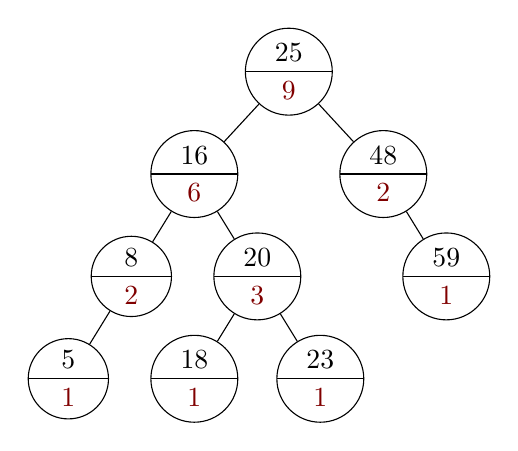
\begin{tikzpicture}[
              level 1/.style={level distance=13mm,sibling distance=24mm},
              level 2/.style={level distance=13mm,sibling distance=16mm},
              level 3/.style={level distance=13mm,sibling distance=16mm},
              level 4/.style={level distance=13mm,sibling distance=16mm},
              every node/.style={minimum width=1em, draw, circle split},
              every lower node part/.style={red!50!black}
            ]
              \node {$25$ \nodepart{lower} $9$}
              child {node {$16$ \nodepart{lower} $6$}
                child {node {$8$ \nodepart{lower} $2$}
                  child {node {$5$ \nodepart{lower} $1$}}
                  child [missing]
                }
                child {node {$20$ \nodepart{lower} $3$}
                  child {node {$18$ \nodepart{lower} $1$}}
                  child {node {$23$ \nodepart{lower} $1$}}
                }
              }
              child {node {$48$ \nodepart{lower} $2$}
                child [missing]
                child {node {$59$ \nodepart{lower} $1$}}
              };
            \end{tikzpicture}
            \caption{
              Order Statistic Tree constructed from $T$. Note each node is \\ augmented
              with an additional field (in red) denoting its $size$.
            }
            \label{fig:bst-size}
          \end{figure}
        \end{minipage}

      \item \label{qst:2b}
        Now, consider the following algorithm, which given a value $x$, computes its {\sc
        Rank}: \vspace{-\baselineskip}
        
        \begin{minipage}{\linewidth}
          \begin{algorithm}[H]
            \caption{$\textsc{Rank}(T,x)$}\label{alg:rank}
            \begin{algorithmic}[1]
              \Require{An augmented and balanced order statistic tree and a value $x$.}
              \Ensure{The position of $x$ (one-indexed!) in the linear sorted list of keys of the tree.}
              \State $r \gets 0$ \Comment{the rank of $x$ in $T$}
              \State $v \gets T.root$
              \While{$v \neq \textsc{nil}$}
                \If{$v.key \leq x$}
                  \If{$v.left \neq \textsc{nil}$}
                    \State $r \gets r + v.left.size + 1$ \Comment{count the \# of elements less than $v$ + $v$ itself}
                  \Else
                    \State $r \gets r + 1$ \Comment{if there isn't a left, just count $v$}
                  \EndIf
                  \If{$v.key = x$}
                    \State \Return{$r$}
                  \EndIf
                  \State $v \gets v.right$ \Comment{explore the right sub-tree}
                \Else
                  \State $v \gets v.left$ \Comment{explore the left sub-tree}
                \EndIf
              \EndWhile
              \State \Return{$r+1$} \Comment{plus one to account for key $x$ not in the tree}
            \end{algorithmic}
          \end{algorithm}
        \end{minipage}

        Suppose $T$ is balanced and augmented. Then at every iteration of the while loop in
        line $3$, \autoref{alg:rank} reduces the problem space by half by carefully choosing
        to explore either the left sub-tree or the right sub-tree. This means \autoref{alg:rank}
        only traverses a single path in $T$ to find the {\sc Rank} of $x$. But any path's length
        in $T$ is bounded by $T$'s height---$\log n$.  So, in the worst case, the length of the
        path traced by \autoref{alg:rank} is exactly $\log n$, which incurs an $\O(\log n)$ cost
        in its runtime.

      \item \label{qst:2c}
        Let $v$ be an arbitrary node in $T$. Then, since the $size$ attribute of $v$ only depends
        on information on $v.left$ and $v.right$, according to the main theorem discussed in class,
        we can maintain the values of $size$ in all nodes of $T$ during $insertion$ and $deletion$
        without affecting the desired $\O(\log n)$ time performance of these operations. Moreover,
        since $size$ only equips $T$ with additional information, the time performance of $search$
        operations remains unchanged.
    \end{enumerate}

  \item \label{qst:3}
    \begin{enumerate}
      \item \label{qst:3a}
        Consider the following algorithm on a balanced binary search tree $T$ whose keys are distinct:
        \vspace{-\baselineskip}
        
        \begin{minipage}{\linewidth}
          \begin{algorithm}[H]
            \caption{$\textsc{Range-Query}(v,x_l,x_r)$}\label{alg:range-query}
            \begin{algorithmic}[1]
              \Require{A node $v$ in $T$ and two real numbers $x_l$ and $x_r$, denoting a range.}
              \Ensure{All keys $x$ stored in $T$ such that $x_l \leq x \leq x_r$.}
              \If{$v \neq \textsc{nil}$}
                \If{$x_l \leq v.key$}
                  \State \Call{Range-Query}{$v.left, x_l, x_r$} \Comment{search left for potential candidates}
                \EndIf
                \If{$x_l \leq v.key \leq x_r$}
                  \State \Call{Print}{$v.key$}
                \EndIf
                \If{$v.key \leq x_r$}
                  \State \Call{Range-Query}{$v.right, x_l, x_r$} \Comment{search right for potential candidates}
                \EndIf
              \EndIf
            \end{algorithmic}
          \end{algorithm}
        \end{minipage}

      \item \label{qst:3b}
        Let $k$ be number of keys of $T$ who fall in the range $[x_l, x_r]$. Then, in either
        execution path, \autoref{alg:range-query} always terminates by reporting exactly $k$
        values of $T$ which means the \textsc{Print} statement in line $6$ is called exactly
        $k$ times---one for each value in the range. Assume this operation is constant. Since
        we have $k$ of those we get an $\O(k)$ cost for reporting/printing the values in the
        range. Added to this cost are the two recursive calls in line $3$ and $9$ that search
        (through only one path!) down to the height of $T$. Now, since $T$ is balanced, the
        two recursive calls incur both an $\O(\log n)$ time cost each.

        So, putting all together, if we let $T(n)$ represent the total time taken for
        \autoref{alg:range-query} to report $k$ of $n$ keys of $T$ in the range $[x_l, x_r]$
        then $T(n) = \O(k) + \O(\log n) + \O(\log n) = \O(k + \log n)$.
    \end{enumerate}

  \item \label{qst:4}
    \begin{enumerate}[ref={(\alph*)}]
      \item \label{qst:4a}
        We augment $T$ as follows: for every node $v$ in $T$ we supplement $v$ with one additional
        field, call it $sum$. This new field will store the cumulative sum of all the values
        descendants of $v$ as well as the value of $v$ itself (see \autoref{fig:bst-sum} for
        details). With this configuration in mind, we wish to maintain the following invariance
        over $sum$: $v.sum = v.left.sum + v.right.sum + v.key$.

        \begin{minipage}{\linewidth}
          \begin{figure}[H]
            \centering
            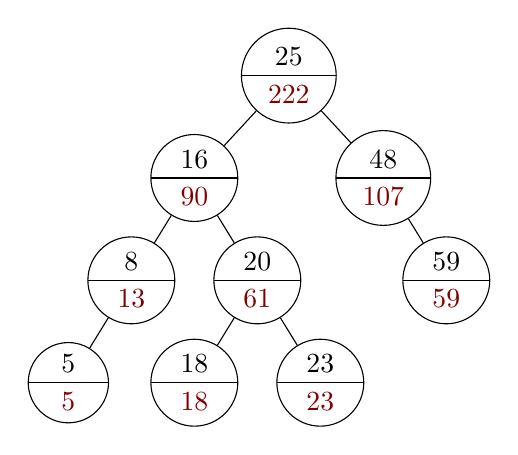
\begin{tikzpicture}[
              level 1/.style={level distance=13mm,sibling distance=24mm},
              level 2/.style={level distance=13mm,sibling distance=16mm},
              level 3/.style={level distance=13mm,sibling distance=16mm},
              level 4/.style={level distance=13mm,sibling distance=16mm},
              every node/.style={minimum width=1em, draw, circle split},
              every lower node part/.style={red!50!black}
            ]
              \node {$25$ \nodepart{lower} $222$}
              child {node {$16$ \nodepart{lower} $90$}
                child {node {$8$ \nodepart{lower} $13$}
                  child {node {$5$ \nodepart{lower} $5$}}
                  child [missing]
                }
                child {node {$20$ \nodepart{lower} $61$}
                  child {node {$18$ \nodepart{lower} $18$}}
                  child {node {$23$ \nodepart{lower} $23$}}
                }
              }
              child {node {$48$ \nodepart{lower} $107$}
                child [missing]
                child {node {$59$ \nodepart{lower} $59$}}
              };
            \end{tikzpicture}
            \caption{
              Augmented and Balanced Binary Search Tree constructed from $T$. \\ Note each
              node $v$ is augmented with an additional field (in red) representing its $sum$.
            }
            \label{fig:bst-sum}
          \end{figure}
        \end{minipage}

      \item \label{qst:4b}
        Now consider the following algorithm, which given a range $[x_l, x_r]$, returns the
        sum of all keys of $T$ in that range: \vspace{-\baselineskip}
        
        \begin{minipage}{\linewidth}
          \begin{algorithm}[H]
            \caption{$\textsc{Range-Sum}(T,x_l,x_r)$}\label{alg:range-sum}
            \begin{algorithmic}[1]
              \Require{An augmented and balanced binary search tree and two real numbers $x_l$ and $x_r$, denoting a range.}
              \Ensure{The sum of all keys of $T$ in the range $[x_l, x_r]$.}
              \State $S_L \gets 0$ \Comment{sum of all keys $< x_l$}
              \State $v \gets T.root$
              \While{$v \neq \textsc{nil}$}
                \If{$v.key < x_l$}
                  \If{$v.left \neq \textsc{nil}$}
                    \State $S_L \gets S_L + v.left.sum + v.key$
                  \Else
                    \State $S_L \gets S_L + v.key$
                  \EndIf
                  \State $v \gets v.right$
                \Else
                  \State $v \gets v.left$
                \EndIf
              \EndWhile
              \State
              \State $S_R \gets 0$ \Comment{sum of all keys $\leq x_r$}
              \State $v \gets T.root$
              \While{$v \neq \textsc{nil}$}
                \If{$v.key \leq x_r$}
                  \If{$v.left \neq \textsc{nil}$}
                    \State $S_R \gets S_R + v.left.sum + v.key$
                  \Else
                    \State $S_R \gets S_R + v.key$
                  \EndIf
                  \State $v \gets v.right$
                \Else
                  \State $v \gets v.left$
                \EndIf
              \EndWhile
              \State
              \State \Return{$S_R - S_L$} \Comment{sum of all keys in $[x_l, x_r]$}
            \end{algorithmic}
          \end{algorithm}
        \end{minipage}

        In analyzing the runtime of \autoref{alg:range-sum}, we notice that there are two almost
        identical pieces in its structure (namely, lines $1$--$14$ and lines $16$--$29$). In both
        of these pieces, we start at the root of the tree and make a decision to either walk left
        or right. We stop until a leaf node is reached. So, the paths traced by these lines
        ($1$--$14$ and $16$--$29$) cannot exceed the height of $T$---$\log n$. This is because every
        time we make a decision to walk left or right, we are effectively narrowing the search space
        by half. But since the search space initially starts with $n$ (the number of nodes in the
        tree), we are restricted to at most $\log n$ steps in that walk until $n$ gets reduced to
        $1$, in which case, we are in the presence of a leaf node. So lines $1$--$14$ and $16$--$29$
        both incur an $\O(\log n)$ cost each, causing the total running time to be:
        \[
          T(n) = \O(\log n) + \O(\log n) + \O(1) = \O(\log n)
        \]
        where the last equality follows from the fact that $\O(1)$ is also $\O(\log n)$, so we get
        $3\O(\log n) = \O(\log n)$ as required!

      \item \label{qst:4c}
        Let $v$ be an arbritrary node in $T$. Then, since---per the $sum$ invariance in part
        \ref{qst:4a}---the $sum$ attribute of $v$ only depends on information on $v$, $v.left$, and
        $v.right$, according to the main theorem discussed in class, we can maintain the values of
        $sum$ in all nodes of $T$ during $insertion$ and $deletion$ without affecting the desired
        $\O(\log n)$ time performance of these operations. Moreover, since $sum$ only equips $T$
        with additional information, the time performance of $search$ operations remains unchanged.
    \end{enumerate}
\end{enumerate}
\end{document}
